\documentclass{standalone}
% translate with >> pdflatex -shell-escape <file>

% This file is an extract of the PGFPLOTS manual, copyright by Christian Feuersaenger.
% 
% Feel free to use it as long as you cite the pgfplots manual properly.
%
% See
%   http://pgfplots.sourceforge.net/pgfplots.pdf
% for the complete manual.
%
% Any required input files (for <plot table> or <plot file> or the table package) can be downloaded
% at
% http://www.ctan.org/tex-archive/graphics/pgf/contrib/pgfplots/doc/latex/
% and
% http://www.ctan.org/tex-archive/graphics/pgf/contrib/pgfplots/doc/latex/plotdata/

\usepackage{pgfplots}
\pgfplotsset{compat=newest}

\pagestyle{empty}

\begin{document}
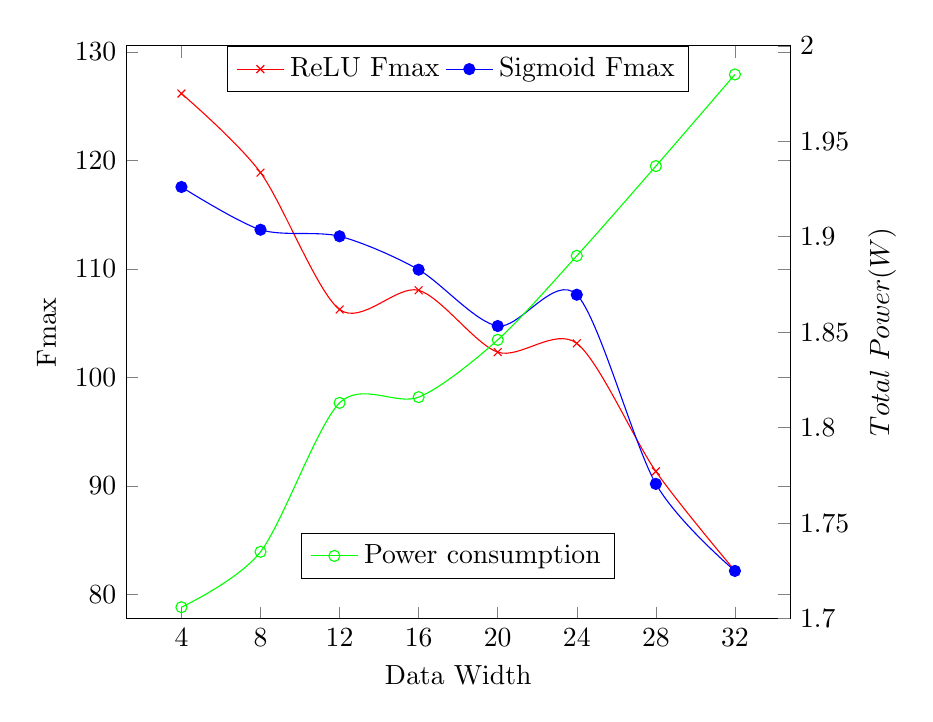
\begin{tikzpicture}
\begin{axis}[
    scale only axis,
	xlabel=Data Width,
    legend style={at={(0.5,1)},
    anchor=north,legend columns=-1},
	ylabel=Fmax,
	xtick=data]
\addplot[smooth,color=red,mark=x] coordinates {
	(4,   126.1670452)
	(8,   118.8777936)
	(12,  106.2586335)
	(16,  108.0263584)
	(20,  102.3227259)
	(24,  103.1353135)
	(28,  91.33254178)
	(32,  82.17602104)
};

\addplot[smooth,color=blue,mark=*] coordinates {
	(4,   117.5502527)
	(8,   113.6105431)
	(12,  113.0071194)
	(16,  109.9263493)
	(20,  104.7339757)
	(24,  107.6194576)
	(28,  90.17945712)
	(32,  82.15576733)
};
\legend{ReLU Fmax,Sigmoid Fmax}
\end{axis}

\begin{axis}[
    scale only axis,
    ymin=1.7,ymax=2,
    axis y line*=right,
    axis x line=none,
    legend style={at={(0.5,0.15)},
    anchor=north,legend columns=-1},
    ylabel=$Total~Power (W)$]
    \addplot[smooth,color=green,mark=o] coordinates {
	(4,   1.706)
	(8,   1.735)
	(12,  1.813)
	(16,  1.816)
	(20,  1.846)
	(24,  1.890)
	(28,  1.937)
	(32,  1.985)
   };
\legend{Power consumption}
\end{axis}


%\end{axis}
\end{tikzpicture}
\end{document}
